\chapter{The QR Algorithm without Shifts}
\label{ch:qr-alg}

Supplementary reading:
\begin{itemize}
  \item \cite{TB} Lecture 28.
  \item \cite{Demmel} Sections 4.4.3 and 4.4.4.
\end{itemize}

\section{Recap}

Last lecture (\Cref{ch:orth-iter}) characterized the matrices whose Schur factorization is a diagonalization, and began computing several eigenpairs at once.
\begin{itemize}
  \item \emph{From Schur factorization to diagonalization} (\Cref{sec:normal}). $A$ is normal, $A^\ast A = AA^\ast$, if and only if $A = Q\Lambda Q^\ast$ with $Q$ unitary (\Cref{thm:normal-diag}). For the Schur factorization $A = QTQ^\ast$, normality of $A$ gives $T^\ast T = TT^\ast$, and comparing $(1,1)$ entries gives $\abs{t_{11}}^2 = \norm{T_{1,:}}^2$: the first row of $T$ is zero off the diagonal. Induction makes $T$ diagonal. In terms of shapes, $T^\ast T = TT^\ast$ says that lower times upper equals upper times lower:
  \begin{center}
  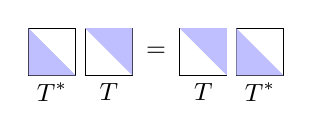
\begin{tikzpicture}[scale=0.6, every node/.style={font=\small}]
    \draw (0,0) rectangle (1,1); \fill[blue!25] (0,1) -- (0,0) -- (1,0) -- cycle;
    \node at (0.5,-0.35) {$T^\ast$};
    \draw (1.2,0) rectangle (2.2,1); \fill[blue!25] (1.2,1) -- (2.2,1) -- (2.2,0) -- cycle;
    \node at (1.7,-0.35) {$T$};
    \node at (2.7,0.5) {$=$};
    \draw (3.2,0) rectangle (4.2,1); \fill[blue!25] (3.2,1) -- (4.2,1) -- (4.2,0) -- cycle;
    \node at (3.7,-0.35) {$T$};
    \draw (4.4,0) rectangle (5.4,1); \fill[blue!25] (4.4,1) -- (4.4,0) -- (5.4,0) -- cycle;
    \node at (4.9,-0.35) {$T^\ast$};
  \end{tikzpicture}
  \end{center}
  The $(1,1)$ entry on the left sees only the first column of $T$, the one on the right the whole first row.
  \item \emph{Orthogonal iteration for two vectors} (\Cref{sec:orth-iter}). Power iteration on $\vec{q}_1, \vec{q}_2$, projecting $\vec{q}_1$ out of $\vec{q}_2$ after each step (\Cref{alg:orth-iter-2}). Then $\vec{q}_1 \to \vec{x}_1$, and once it has converged,
  \begin{equation}
    \vec{q}_2^{(k)} = (I - \vec{x}_1\vec{x}_1^\ast)A(I - \vec{x}_1\vec{x}_1^\ast)\vec{q}_2^{(k-1)}
  \end{equation}
  up to normalization. This matrix has the eigenpairs $(\lambda_i, (I - \vec{x}_1\vec{x}_1^\ast)\vec{x}_i)$ for $i \ge 2$:
  \begin{equation}
    (I - \vec{x}_1\vec{x}_1^\ast)A(I - \vec{x}_1\vec{x}_1^\ast)\vec{x}_i = \lambda_i(I - \vec{x}_1\vec{x}_1^\ast)\vec{x}_i.
  \end{equation}
  Hence $\vec{q}_2^{(k)} \to (I - \vec{x}_1\vec{x}_1^\ast)\vec{x}_2$, which differs from $\vec{x}_2$ unless $\vec{x}_1 \perp \vec{x}_2$ (as for normal $A$). What converges is the subspace, $\spn(\vec{q}_1, \vec{q}_2) \to \spn(\vec{x}_1, \vec{x}_2)$.
  \item \emph{Orthogonal iteration for a general number of vectors} (\Cref{sec:orth-iter-general}). With $r$ columns, the projection step becomes a reduced QR factorization (\Cref{alg:orth-iter}):
\begin{lstlisting}
for k = 1:iterations
    Q = A*Q
    Q, R = qr(Q)
end
\end{lstlisting}
\end{itemize}

\section{Schur and Eigendecomposition}
\label{sec:schur-eig}

Throughout this lecture we consider
\begin{equation}
  A = X\Lambda X^{-1}, \qquad \abs{\lambda_1} > \abs{\lambda_2} > \dots > \abs{\lambda_m},
  \label{eq:qr-alg-assumption}
\end{equation}
i.e., $A$ is diagonalizable and its eigenvalues have distinct moduli.

This assumption is \emph{generic}: it holds for all matrices except a set that can be removed by an arbitrarily small perturbation. The reason is that every $A$ has a Schur factorization $A = QTQ^\ast$ with the eigenvalues on the diagonal of $T$ (\Cref{thm:schur}). We can add a small perturbation to the diagonal of $T$, and hence to $A$, such that
\begin{equation}
  \tilde{A} \defeq Q\bigl(T + \diag(\eps_1, \dots, \eps_m)\bigr)Q^\ast = A + Q\diag(\eps_1, \dots, \eps_m)Q^\ast
\end{equation}
has eigenvalues of distinct magnitude. Indeed, $\tilde{A}$ is in Schur form with diagonal entries $t_{ii} + \eps_i$, these are its eigenvalues, and the $\eps_i$ can be chosen to make their moduli distinct. The perturbation is small, $\norm{\tilde{A} - A} = \max_i\abs{\eps_i}$, since $Q$ is unitary. Distinct eigenvalues imply diagonalizability, so $\tilde{A}$ satisfies \cref{eq:qr-alg-assumption}. Conversely, eigenvalues depend continuously on the matrix, so the strict inequalities survive small perturbations of $\tilde{A}$.

\begin{remark}[Real Matrices (SUPPLEMENT)]
  The perturbation above is complex in general. For real $A$, non-real eigenvalues come in conjugate pairs $\lambda, \overline{\lambda}$ with $\abs{\lambda} = \abs{\overline{\lambda}}$, and a small real perturbation keeps them a conjugate pair. So among real matrices, \cref{eq:qr-alg-assumption} is not generic; it fails on an open set, e.g., near every rotation of $\R^2$ by an angle $\theta \notin \{0, \pi\}$.
\end{remark}

Now, given $A = X\Lambda X^{-1}$, how do we compute its Schur form? Take a QR factorization of the eigenvector matrix, $X = QR$. Since $X$ is invertible, so is $R$, and
\begin{equation}
  X = QR \quad\Longrightarrow\quad A = QR\Lambda R^{-1}Q^\ast = Q\underbrace{(R\Lambda R^{-1})}_{\text{upper triangular}}Q^\ast.
  \label{eq:schur-from-eig}
\end{equation}
Indeed, $R^{-1}$ is upper triangular, products of upper triangular matrices are upper triangular, and the diagonal of $R\Lambda R^{-1}$ is $r_{ii}\lambda_ir_{ii}^{-1} = \lambda_i$. So \cref{eq:schur-from-eig} is a Schur factorization of $A$, with the eigenvalues on the diagonal of $T = R\Lambda R^{-1}$ in the same order as in $\Lambda$.

Since $R$ is upper triangular, $\vec{x}_j = \sum_{i \le j}r_{ij}\vec{q}_i$ only involves the first $j$ columns of $Q$, and since $R$ is invertible the converse holds as well. Hence
\begin{equation}
  \spn(\vec{q}_1, \dots, \vec{q}_j) = \spn(\vec{x}_1, \dots, \vec{x}_j), \qquad j = 1, \dots, m:
  \label{eq:schur-nested}
\end{equation}
the Schur vectors span the same nested invariant subspaces as the eigenvectors. This is not an algorithm, since it needs $X$, but it identifies the target: the rest of the lecture shows that orthogonal iteration converges to these subspaces without knowing $X$.
\section{Convergence of Orthogonal Iteration}
\label{sec:orth-iter-conv}

How should we think about the convergence of orthogonal iteration (\Cref{alg:orth-iter})? Let $Q_k \in \K^{m \times p}$ be the iterate after $k$ steps, starting from $Q_0$ with $p$ orthonormal columns. Let $A = X\Lambda X^{-1}$ be diagonalizable with its eigenvalues ordered by modulus, $\abs{\lambda_1} \ge \abs{\lambda_2} \ge \dots \ge \abs{\lambda_m}$. For this section we need less than \cref{eq:qr-alg-assumption}: it suffices that there is a gap after the $p$th eigenvalue,
\begin{equation}
  \abs{\lambda_p} > \abs{\lambda_{p+1}}.
  \label{eq:orth-iter-gap}
\end{equation}
As in \Cref{ch:orth-iter}, track the subspace $\spn(Q_k)$, the span of the columns, rather than the individual columns.

The QR step does not change the column space, so $\spn(Q_{k+1}) = \spn(AQ_k)$, and unrolling the recursion,
\begin{equation}
  \spn(Q_{k+1}) = \spn(AQ_k) = \dots = \spn(A^{k+1}Q_0) = \spn(X\Lambda^{k+1}X^{-1}Q_0).
\end{equation}
Pull out the factor $\lambda_p^{k+1}$, which does not change the span (note $\lambda_p \ne 0$, since $\abs{\lambda_p} > \abs{\lambda_{p+1}} \ge 0$ by \cref{eq:orth-iter-gap}):
\begin{equation}
  \spn(Q_{k+1}) = \spn\left(\lambda_p^{k+1}X\begin{bmatrix}
    (\lambda_1/\lambda_p)^{k+1} & & & & \\
    & \ddots & & & \\
    & & 1 & & \\
    & & & \ddots & \\
    & & & & (\lambda_m/\lambda_p)^{k+1}
  \end{bmatrix}X^{-1}Q_0\right),
\end{equation}
with the $1$ in position $(p, p)$. By the ordering of the eigenvalues and the gap \cref{eq:orth-iter-gap},
\begin{equation}
  \abs{\lambda_i/\lambda_p} \ge 1 \quad\text{for } i \le p, \qquad \abs{\lambda_i/\lambda_p} < 1 \quad\text{for } i > p.
\end{equation}
So the first $p$ rows of $(\Lambda/\lambda_p)^{k+1}X^{-1}Q_0$ do not decay, while the last $m - p$ rows are scaled by factors that tend to zero. Split accordingly:
\begin{equation}
  \left(\Lambda/\lambda_p\right)^{k+1}X^{-1}Q_0 = \begin{bmatrix} V_k \\ W_k \end{bmatrix}, \qquad V_k \in \K^{p \times p}, \quad W_k \in \K^{(m-p) \times p}, \qquad W_k \xrightarrow{k \to \infty} 0,
\end{equation}
where $W_k$ decays like $\abs{\lambda_{p+1}/\lambda_p}^{k+1}$. Splitting the columns of $X$ in the same way, $X = [X_p\ \tilde{X}_p]$ with $X_p = [\vec{x}_1 \cdots \vec{x}_p]$ the first $p$ eigenvectors, gives
\begin{equation}
  \spn(Q_{k+1}) = \spn(X\Lambda^{k+1}X^{-1}Q_0) = \spn(X_pV_k + \tilde{X}_pW_k) \xrightarrow{k \to \infty} \spn(X_p).
  \label{eq:orth-iter-split}
\end{equation}
So $\spn(Q_k)$ converges to $\spn(\vec{x}_1, \dots, \vec{x}_p)$, the invariant subspace of the $p$ dominant eigenvectors.

To make the limit precise (SUPPLEMENT), write $B \defeq X^{-1}Q_0 = \left[\begin{smallmatrix} B_1 \\ B_2 \end{smallmatrix}\right]$, the coordinates of $Q_0$ in the eigenvector basis, with $B_1 \in \K^{p \times p}$, and $\Lambda = \diag(\Lambda_1, \Lambda_2)$ with $\Lambda_1 = \diag(\lambda_1, \dots, \lambda_p)$. Then
\begin{equation}
  V_k = (\Lambda_1/\lambda_p)^{k+1}B_1, \qquad W_k = (\Lambda_2/\lambda_p)^{k+1}B_2.
\end{equation}
Assume $B_1$ is invertible, i.e., $Q_0$ has a nonzero component in every direction $\vec{x}_1, \dots, \vec{x}_p$; this is the analogue of $\vec{x}_1^\ast\vec{q}^{(0)} \ne 0$ for power iteration and holds with probability one for random $Q_0$. Then $V_k$ is invertible, and multiplying by $V_k^{-1}$ on the right does not change the span:
\begin{equation}
  \spn(X_pV_k + \tilde{X}_pW_k) = \spn\bigl(X_p + \tilde{X}_pW_kV_k^{-1}\bigr).
\end{equation}
Since $V_k^{-1} = B_1^{-1}(\lambda_p\Lambda_1^{-1})^{k+1}$ and $\abs{\lambda_p/\lambda_i} \le 1$ for $i \le p$, we get $\norm{V_k^{-1}} \le \norm{B_1^{-1}}$, so
\begin{equation}
  \norm{\tilde{X}_pW_kV_k^{-1}} \le \norm{\tilde{X}_p}\norm{B_2}\norm{B_1^{-1}}\abs{\frac{\lambda_{p+1}}{\lambda_p}}^{k+1} \longrightarrow 0.
\end{equation}
The subspace converges at the rate $\abs{\lambda_{p+1}/\lambda_p}$, the gap between the last eigenvalue we keep and the first one we discard.

\section{Convergence to Schur Factorization}
\label{sec:conv-schur}

Now run orthogonal iteration with $p = m$, i.e., on a full orthonormal basis, starting from $Q_0 = I$.

\begin{theorem}[Orthogonal Iteration Converges to Schur Form]
  \label{thm:orth-iter-schur}
  Consider orthogonal iteration (\Cref{alg:orth-iter}) on $A = X\Lambda X^{-1}$ with $p = m$ and $Q_0 = I$. If all eigenvalues of $A$ have distinct absolute values, $\abs{\lambda_1} > \dots > \abs{\lambda_m}$, and the leading blocks $(X^{-1})_{1:j,1:j}$ have full rank for $j = 1, \dots, m$, then
  \begin{equation}
    T_k \defeq Q_k^\ast AQ_k
  \end{equation}
  converges to the Schur form of $A$: its strictly lower triangular part tends to zero and its diagonal tends to $(\lambda_1, \dots, \lambda_m)$.
\end{theorem}

Note that the condition is on the leading blocks of $X^{-1}$, not of $X$; the two are not equivalent, although the condition is sometimes stated with $X_{1:j,1:j}$ (e.g., \cite[Thm.~4.8]{Demmel}). The argument of \Cref{sec:orth-iter-conv} needs a condition on $X^{-1}Q_0 = X^{-1}$: for $j$ columns, the block $B_1$ consists of the first $j$ rows and columns, $(X^{-1})_{1:j,1:j}$. Requiring instead that $X_{1:j,1:j}$ have full rank for all $j$ is not enough. For
\begin{equation}
  X = \begin{bmatrix} 1 & 1 \\ 1 & 0 \end{bmatrix}, \qquad X^{-1} = \begin{bmatrix} 0 & 1 \\ 1 & -1 \end{bmatrix},
\end{equation}
$X_{1:1,1:1} = 1$ and $X$ are nonsingular, but $(X^{-1})_{11} = 0$: the starting vector $\vec{e}_1 = \vec{x}_2$ is itself an eigenvector, has no component along $\vec{x}_1$, and in exact arithmetic $\vec{q}_1^{(k)} = \vec{x}_2$ forever. By Jacobi's identity for complementary minors, $\det (X^{-1})_{1:j,1:j} = \det X_{j+1:m,j+1:m}/\det X$, so the correct condition can equally be stated as: the trailing blocks $X_{j+1:m,j+1:m}$ are nonsingular. Equivalently, $X^{-1}$ has an LU factorization without pivoting. For normal $A = Q\Lambda Q^\ast$ the distinction disappears: $X = Q$ is unitary, $X^{-1} = Q^\ast$, and $(Q^\ast)_{1:j,1:j} = (Q_{1:j,1:j})^\ast$, so the leading blocks of $X^{-1}$ are nonsingular exactly when those of $X$ are. This is why Trefethen and Bau, who treat real symmetric $A = Q\Lambda Q^\T$, can state the condition as ``all leading principal submatrices of $Q$ are nonsingular''~\cite[Thm.~28.4]{TB}. For non-normal $A$ the example above shows that only the condition on $X^{-1}$ is correct.

\begin{proof}[Proof sketch]
  Fix $p \in \{1, \dots, m - 1\}$ and split the columns of $Q_k$ after the $p$th (here $p$ is a split index; $Q_k$ has all $m$ columns):
  \begin{equation}
    Q_k = [\bar{Q}_k\ \tilde{Q}_k], \qquad \bar{Q}_k \in \K^{m \times p}.
  \end{equation}
  Then
  \begin{equation}
    T_k = Q_k^\ast AQ_k = \begin{bmatrix} \bar{Q}_k^\ast A\bar{Q}_k & \bar{Q}_k^\ast A\tilde{Q}_k \\ \tilde{Q}_k^\ast A\bar{Q}_k & \tilde{Q}_k^\ast A\tilde{Q}_k \end{bmatrix}.
  \end{equation}
  Column $j$ of a QR factorization depends only on the first $j$ columns of the factored matrix, so $\bar{Q}_k$ is exactly the iterate of orthogonal iteration with $p$ columns started from $\bar{Q}_0 = I_{:,1:p}$. By \Cref{sec:orth-iter-conv},
  \begin{equation}
    \spn(\bar{Q}_k) \longrightarrow \spn(\vec{x}_1, \dots, \vec{x}_p).
  \end{equation}
  Applying $A$,
  \begin{equation}
    \spn(A\bar{Q}_k) \longrightarrow \spn(A[\vec{x}_1 \cdots \vec{x}_p]) = \spn([\vec{x}_1 \cdots \vec{x}_p]),
  \end{equation}
  where the equality holds because $A[\vec{x}_1 \cdots \vec{x}_p] = [\vec{x}_1 \cdots \vec{x}_p]\diag(\lambda_1, \dots, \lambda_p)$ and $\lambda_1, \dots, \lambda_p \ne 0$ (as $\abs{\lambda_p} > \abs{\lambda_{p+1}} \ge 0$): the span of the dominant eigenvectors is invariant under $A$. So the columns of $A\bar{Q}_k$ lie (asymptotically) in $\spn(\bar{Q}_k)$, while the columns of $\tilde{Q}_k$ are orthogonal to $\spn(\bar{Q}_k)$. Hence
  \begin{equation}
    \tilde{Q}_k^\ast A\bar{Q}_k \longrightarrow 0.
  \end{equation}
  More precisely, $\tilde{Q}_k^\ast\bar{Q}_k = 0$ gives $\tilde{Q}_k^\ast A\bar{Q}_k = \tilde{Q}_k^\ast(I - \bar{Q}_k\bar{Q}_k^\ast)A\bar{Q}_k$, and $(I - \bar{Q}_k\bar{Q}_k^\ast)A\bar{Q}_k$, the part of $A\bar{Q}_k$ outside $\spn(\bar{Q}_k)$, tends to zero.

  The lower left block of the split after column $p$ contains the entries $(i, j)$ with $i > p \ge j$. Every strictly lower triangular entry $(i, j)$, $i > j$, lies in this block for $p = j$, so the argument holds for all subdiagonal blocks, and letting $p$ range over $1, \dots, m - 1$ shows that
  \begin{equation}
    T_k = Q_k^\ast AQ_k \longrightarrow \text{upper triangular}.
  \end{equation}
  For the diagonal (SUPPLEMENT): $\bar{Q}_k^\ast A\bar{Q}_k$ is the matrix of $A$ restricted to $\spn(\bar{Q}_k) \to \spn(\vec{x}_1, \dots, \vec{x}_p)$, so its eigenvalues tend to $\lambda_1, \dots, \lambda_p$, as in \Cref{prop:orth-iter-2x2}. Since this block becomes upper triangular, its diagonal holds these eigenvalues, and comparing $p$ with $p - 1$ shows that the $p$th diagonal entry of $T_k$ tends to $\lambda_p$.
\end{proof}

\section{Basic QR Iteration}
\label{sec:basic-qr}

Orthogonal iteration allows computing
\begin{equation}
  T_k \defeq Q_k^\ast AQ_k,
\end{equation}
which converges to the triangular factor of a Schur factorization (\Cref{thm:orth-iter-schur}).

Computing $T_{k+1}$ this way requires $Q_k$ and a matrix-matrix product with $A$. Can we instead derive an iteration $T_k \to T_{k+1}$ that works with the $T$'s alone? Observe that
\begin{equation}
  T_k = Q_k^\ast AQ_k, \qquad T_{k+1} = Q_{k+1}^\ast AQ_{k+1}.
\end{equation}
One step of orthogonal iteration is the QR factorization $Q_{k+1}R_{k+1} = AQ_k$. Multiplying by $Q_{k+1}^\ast$ on the left and by $Q_k^\ast$ on the right (here $p = m$, so $Q_k$ is square and $Q_kQ_k^\ast = I$),
\begin{equation}
  Q_{k+1}R_{k+1} = AQ_k \quad\Longrightarrow\quad R_{k+1}Q_k^\ast = Q_{k+1}^\ast A.
\end{equation}
Substituting the first form into $T_k$ and the second into $T_{k+1}$,
\begin{equation}
  T_k = Q_k^\ast(Q_{k+1}R_{k+1}), \qquad T_{k+1} = (R_{k+1}Q_k^\ast)Q_{k+1}.
  \label{eq:qr-iter-derivation}
\end{equation}
Both expressions contain the same product $Q_k^\ast Q_{k+1}$. Naming it,
\begin{equation}
  U_{k+1} \defeq Q_k^\ast Q_{k+1}: \qquad T_k = U_{k+1}R_{k+1}, \qquad T_{k+1} = R_{k+1}U_{k+1}.
  \label{eq:qr-iter-UR}
\end{equation}
Here $U_{k+1}$ is unitary, since $U_{k+1}^\ast U_{k+1} = Q_{k+1}^\ast Q_kQ_k^\ast Q_{k+1} = I$, and $R_{k+1}$ is upper triangular. So $T_k = U_{k+1}R_{k+1}$ is a QR factorization of $T_k$, and $T_{k+1}$ is obtained by multiplying its factors in reverse order:
\begin{equation}
  T_k = U_{k+1}R_{k+1} \quad\longrightarrow\quad T_{k+1} = R_{k+1}U_{k+1}.
\end{equation}
In short: factor as $QR$, multiply back as $RQ$. Neither $A$ nor $Q_k$ appears. Note that $T_{k+1} = R_{k+1}U_{k+1} = U_{k+1}^\ast(U_{k+1}R_{k+1})U_{k+1} = U_{k+1}^\ast T_kU_{k+1}$ is unitarily similar to $T_k$, so every $T_k$ has the eigenvalues of $A$.

Starting orthogonal iteration from $Q_0 = I$ gives $T_0 = Q_0^\ast AQ_0 = A$, so the iteration starts from $A$ itself.

\begin{algorithm}[H]
  \caption{Basic QR iteration (QR algorithm without shifts).}
  \label{alg:basic-qr}
  \begin{algorithmic}[1]
    \Require $A \in \K^{m \times m}$
    \State $T \gets A$
    \For{$k = 1, \dots, \mathrm{maxiter}$}
      \State $UR \gets T$ \Comment{QR factorization}
      \State $T \gets RU$
    \EndFor
    \State \Return $\diag(T)$ \Comment{approximate eigenvalues $\lambda_1, \dots, \lambda_m$}
  \end{algorithmic}
\end{algorithm}

By \Cref{thm:orth-iter-schur}, $T$ converges to upper triangular form with the eigenvalues on its diagonal, ordered by decreasing modulus. A library QR routine need not return the same factors as orthogonal iteration: for invertible $T$, QR factors are unique only up to signs (phases) of the columns of $U$ and rows of $R$~(\Cref{ch:qr}). Any choice gives $T_{k+1} = U^\ast T_kU$, and different choices produce iterates that differ by a diagonal unitary similarity $D^\ast T_kD$, which leaves the diagonal and the moduli of all entries unchanged.

\paragraph{How to obtain $Q$?} \Cref{alg:basic-qr} returns only the eigenvalues; the Schur vectors $Q_k$ of orthogonal iteration never appear. They can be recovered from the factors $U$, since by definition
\begin{equation}
  U_{k+1} = Q_k^\ast Q_{k+1}.
\end{equation}
The product of the $U$'s telescopes: since $Q_kQ_k^\ast = I$ and $Q_0 = I$,
\begin{equation}
  U_1U_2\cdots U_{k+1} = (Q_0^\ast Q_1)(Q_1^\ast Q_2)\cdots(Q_k^\ast Q_{k+1}) = Q_0^\ast Q_{k+1} = Q_{k+1}.
\end{equation}
So to obtain the Schur vectors, start from $Q \gets I$ and accumulate $Q \gets QU$ after each QR factorization in \Cref{alg:basic-qr}; on return, $A \approx QTQ^\ast$.

The factors $U_k$ have a simple interpretation. Close to convergence, $Q_{k+1} \approx Q_k$ up to the phases of the columns, so $U_{k+1} = Q_k^\ast Q_{k+1}$ is a small rotation: it is close to a diagonal unitary matrix $D$. This can also be seen from $T_k = U_{k+1}R_{k+1}$. Once $T_k$ is nearly upper triangular, $U_{k+1} = T_kR_{k+1}^{-1}$ is nearly upper triangular and unitary, hence nearly diagonal. With the normalization $r_{ii} > 0$ we get $D \approx \diag(\lambda_1/\abs{\lambda_1}, \dots, \lambda_m/\abs{\lambda_m})$, so $D = I$ only when all eigenvalues are positive. A negative eigenvalue flips the sign of the corresponding column of $Q_k$ in every step, exactly as in power iteration. Up to these phases, the $U_k$ form a sequence of rotational corrections that transform $Q_0 = I$ into the Schur vectors $Q$, with large corrections in the first steps and ever smaller ones as $T_k$ approaches triangular form.

\begin{remark}[Julia]
  For square $T$ the implicit $Q$ returned by \texttt{qr} (\Cref{ch:qr}) can be multiplied directly, so the pitfall of \Cref{ch:orth-iter} does not arise:
\begin{lstlisting}
T = copy(A); Q = Matrix(1.0I, m, m)
for k = 1:maxiter
    F = qr(T)
    T = F.R * F.Q
    Q = Q * F.Q
end
\end{lstlisting}
\end{remark}

\section{(SUPPLEMENT) Further Topics}
\label{sec:qr-alg-supp}

\paragraph{The QR algorithm factors the powers of $A$.} Let $\underline{R}_k \defeq R_kR_{k-1}\cdots R_1$, the product of the triangular factors of orthogonal iteration started from $Q_0 = I$. Then
\begin{equation}
  A^k = Q_k\underline{R}_k, \qquad T_k = Q_k^\ast AQ_k, \qquad Q_k = U_1U_2\cdots U_k.
  \label{eq:qr-alg-powers}
\end{equation}
The first identity follows by induction, $A^k = A\,Q_{k-1}\underline{R}_{k-1} = Q_kR_k\underline{R}_{k-1} = Q_k\underline{R}_k$, and $\underline{R}_k$ is upper triangular as a product of upper triangular matrices. So the QR algorithm computes a QR factorization of $A^k$ without ever forming $A^k$, whose columns would all be nearly parallel to $\vec{x}_1$. The two identities in \cref{eq:qr-alg-powers} explain the whole algorithm~\cite[Lecture~28]{TB}. The first says that the leading $j$ columns of $Q_k$ are an orthonormal basis of the span of the leading $j$ columns of $A^k$: this is simultaneous power iteration on $\vec{e}_1, \dots, \vec{e}_m$. The second says that the diagonal entries $(T_k)_{jj} = \vec{q}_j^{(k)\ast}A\vec{q}_j^{(k)}$ are Rayleigh quotients. For Hermitian $A$, they therefore converge twice as fast as the columns of $Q_k$ (\Cref{ch:eigen}).

\paragraph{Simultaneous inverse iteration.} If $A$ is invertible, inverting and taking the adjoint of $A^k = Q_k\underline{R}_k$ gives
\begin{equation}
  (A^\ast)^{-k} = \bigl(\underline{R}_k^{-1}Q_k^\ast\bigr)^\ast = Q_k\underline{R}_k^{-\ast},
\end{equation}
with $\underline{R}_k^{-\ast}$ lower triangular. Let $P$ be the permutation that reverses the order of the rows, $P^2 = I$. Reversing both the rows and the columns of a lower triangular matrix makes it upper triangular, so
\begin{equation}
  (A^\ast)^{-k}P = (Q_kP)\bigl(P\underline{R}_k^{-\ast}P\bigr)
\end{equation}
is a QR factorization of $(A^\ast)^{-k}P$. Hence $Q_kP$, i.e., $Q_k$ with its columns in reverse order, is what orthogonal iteration with $(A^\ast)^{-1}$ produces from $Q_0 = P$. In particular, the last column of $Q_k$ is the result of $k$ steps of inverse iteration (\Cref{alg:inverse}) with $A^\ast$, started from $\vec{e}_m$. It converges at the rate $\abs{\lambda_m/\lambda_{m-1}}$ to an eigenvector $\vec{y}_m$ of $A^\ast$ for $\overline{\lambda_m}$. This is a left eigenvector of $A$, $\vec{y}_m^\ast A = \lambda_m\vec{y}_m^\ast$, and it is orthogonal to $\vec{x}_1, \dots, \vec{x}_{m-1}$, consistent with \cref{eq:schur-nested}. So the QR algorithm runs power iteration in its first column and inverse iteration in its last column at the same time. For real symmetric $A$, $A^\ast = A$; see~\cite[Lecture~29]{TB}.

\paragraph{Convergence rates of individual entries.} By \Cref{sec:orth-iter-conv}, the block $(T_k)_{p+1:m,1:p}$ below and to the left of the split after column $p$ decays like $\abs{\lambda_{p+1}/\lambda_p}^k$. In particular, the subdiagonal entry $(T_k)_{j+1,j}$ decays like $\abs{\lambda_{j+1}/\lambda_j}^k$, and the diagonal entry $(T_k)_{pp}$ converges to $\lambda_p$ like $\max(\abs{\lambda_{p+1}/\lambda_p}^k, \abs{\lambda_p/\lambda_{p-1}}^k)$~\cite[\S4.4.3]{Demmel}. The overall rate is the worst ratio $\max_j\abs{\lambda_{j+1}/\lambda_j}$~\cite[Thm.~28.4]{TB}, so two eigenvalues of nearly equal modulus make the unshifted algorithm arbitrarily slow. For example, for $\Lambda = \diag(30, 6, 2, 1)$ and a random $X$ with $\kappa(X) \approx 20$, after $19$ steps the subdiagonal entries are about $7 \cdot 10^{-13}$, $1 \cdot 10^{-9}$, and $5 \cdot 10^{-6}$~\cite[Example~4.5]{Demmel}, in line with $(1/5)^{19} \approx 5 \cdot 10^{-14}$, $(1/3)^{19} \approx 9 \cdot 10^{-10}$, and $(1/2)^{19} \approx 2 \cdot 10^{-6}$ up to constants. The most important block is the last row, $(T_k)_{m,1:m-1}$, which decays like $\abs{\lambda_m/\lambda_{m-1}}^k$. Once it is below a tolerance such as $\epsm\norm{A}$, we accept $(T_k)_{mm}$ as an eigenvalue and continue on the leading $(m-1) \times (m-1)$ block (deflation).

\paragraph{Eigenvalues of equal modulus.} Without a gap $\abs{\lambda_p} > \abs{\lambda_{p+1}}$, the block at the split after column $p$ has no reason to decay. In the extreme case of a unitary $A$, all eigenvalues have modulus $1$. Its QR factorization is $A = A \cdot I$, so $T_1 = I \cdot A = A$, and the iteration does not move at all~\cite[Example~4.6]{Demmel}. An example is $A = \left[\begin{smallmatrix} 0 & 1 \\ 1 & 0 \end{smallmatrix}\right]$, with eigenvalues $\pm 1$. The generic case for real matrices is a pair of complex conjugate eigenvalues $\lambda, \overline{\lambda}$ (see the remark in \Cref{sec:schur-eig}). For real $A$, all $U_k$, $R_k$, and $T_k$ are real, so $T_k$ cannot converge to a triangular matrix with non-real diagonal entries. The splits between eigenvalues of different moduli still have a gap, however, so the corresponding blocks still decay (under the analogous rank conditions). If the only ties in modulus come from conjugate pairs, $T_k$ converges to a block upper triangular matrix with $1 \times 1$ and $2 \times 2$ diagonal blocks, i.e., to the real Schur form (\Cref{thm:real-schur}). The entries of each $2 \times 2$ block keep changing from step to step, but its eigenvalues converge to $\lambda, \overline{\lambda}$.

\paragraph{Why shifts help.} The shifted matrix $A - \sigma I = Q(T - \sigma I)Q^\ast$ has the same Schur vectors as $A$ and the eigenvalues $\lambda_i - \sigma$. Running the QR algorithm on it therefore converges at the rates $\abs{\lambda_{j+1} - \sigma}/\abs{\lambda_j - \sigma}$, with the eigenvalues now ordered by their distance from $\sigma$. If $\sigma$ is close to an eigenvalue $\lambda$, the last row decays at the rate $\abs{\lambda - \sigma}/\min_{\lambda_j \ne \lambda}\abs{\lambda_j - \sigma}$, which is nearly zero. The shift may change from step to step, and it need not be undone:
\begin{equation}
  T_k - \sigma_kI = U_{k+1}R_{k+1}, \qquad T_{k+1} = R_{k+1}U_{k+1} + \sigma_kI = U_{k+1}^\ast T_kU_{k+1},
\end{equation}
so $T_{k+1}$ is still unitarily similar to $A$~\cite[\S4.4.4]{Demmel}. By the previous paragraphs, the last column of $Q_k$ then performs shifted inverse iteration. The natural choice $\sigma_k = (T_k)_{mm}$, the Rayleigh quotient of that column, turns it into a version of Rayleigh quotient iteration (\Cref{alg:rqi}), with cubic convergence for real symmetric $A$~\cite[Lecture~29]{TB}. Shifts also break ties in modulus: for $A = \left[\begin{smallmatrix} 0 & 1 \\ 1 & 0 \end{smallmatrix}\right]$ and real $\sigma \ne 0$, $\abs{1 - \sigma} \ne \abs{-1 - \sigma}$. There, however, $(T_k)_{mm} = 0$ gives no shift at all, which is why practical codes use a more robust shift. Fast convergence alone is not enough, since each step of \Cref{alg:basic-qr} still costs $O(m^3)$. Reducing this cost with a Hessenberg reduction, and adding shifts, is the subject of \Cref{ch:hessenberg-qr}.
